\documentclass[conference]{IEEEtran}
\IEEEoverridecommandlockouts
% The preceding line is only needed to identify funding in the first footnote. If that is unneeded, please comment it out.
\usepackage{cite}
\usepackage{amsmath,amssymb,amsfonts}
\usepackage{multirow}
\usepackage{algorithm}
\usepackage{algorithmic}
\usepackage{float}
\usepackage{siunitx} % Standard package for SI units
\usepackage{graphicx}
\usepackage{tikz}
\usetikzlibrary{arrows.meta, positioning, fit, calc}
\usepackage{textcomp}
\usepackage{xcolor}
\def\BibTeX{{\rm B\kern-.05em{\sc i\kern-.025em b}\kern-.08em
    T\kern-.1667em\lower.7ex\hbox{E}\kern-.125emX}}
\begin{document}

\title{Tiny Acceleration of Liquid Foundation Models}

\author{\IEEEauthorblockN{Jacopo Marchesin}
\IEEEauthorblockA{\textit{DISI} \\
\textit{University of Trento}\\
Trento, Italy \\
marchesin.jacopo772@gmail.com}
\and
\IEEEauthorblockN{Roberto Passerone}
\IEEEauthorblockA{\textit{DISI} \\
\textit{University of Trento}\\
Trento, Italy \\
roberto.passerone@unitn.it}
\and
\IEEEauthorblockN{Danilo Pau}
\IEEEauthorblockA{\textit{System Research and Applications} \\
\textit{STMicroelectronics}\\
Agrate Brianza, Italy \\
danilo.pau@st.com}
}

\maketitle

\begin{abstract}
This work presents a systems-driven approach to enabling conversational audio inference on resource-constrained edge devices. This is achieved through a custom FPGA accelerator for the LFM2.5-1.2B-Thinking model by Liquid AI designed to offload the heaviest part of inference to reduce latency and energy consumption. The proposed implementation enables a comprehensive evaluation of the interaction between computation and data movement in transformer feed-forward layers under edge constraints. Results show a significant reduction in energy consumption while maintaining compatibility with existing inference frameworks. These findings demonstrate that selectively accelerating feed-forward components provides an effective pathway toward conversational-level performance on embedded platforms.
\end{abstract}

\begin{IEEEkeywords}
FPGA, Edge AI, LFM2, Hardware Acceleration
\end{IEEEkeywords}

\section{Introduction}\label{introd}
The rapid growth of intelligent sensing devices is shifting AI from power hungry data centers and cloud-centric systems to low power edge platforms where perception, generation, reasoning, and control occur near the data source under challenging latency, energy, and privacy constraints \cite{reddi2025generative}. 

About perception, TinyML was the initial step for edge intelligence, which demonstrated inference was feasible on microcontrollers (MCUs) using hyper-parameterized CNN and RNN models \cite{10177729} \cite{mi13060851}. Since then, the edge evolved to embrace Generative Edge AI. Modern Edge AI is built on heterogeneously quantized Transformer architectures, including small language models (SLMs), which seek to retain useful generative and reasoning capabilities under tight resource (memory and computation) budgets \cite{technologies12060081, electronics14173468}. Techniques such as deep quantization, pruning, knowledge distillation, and hardware-aware neural architecture design have become central to reconciling model accuracy with deployability \cite{s25103191}.
Delivering real-time responsiveness requires tight integration of models, algorithms, and low power hardware. 

In this landscape, conversational audio emerges because it is a profound human need \cite{Seltzer2012} and also a desirable target for edge deployment. Conversational systems impose stringent real-time constraints that benefit from the elimination of network latency. Unlike vision workloads, audio pipelines can be implemented as modular stages like wake-word detection and automatic speech recognition. These components typically operate on low-dimensional temporal features and can be aggressively quantized without prohibitive quality loss. Furthermore, conversational audio frequently contains biometric identifiers and sensitive spoken information, making local processing desirable from both privacy and regulatory perspectives.

This paper begins by formally defining the objectives of this work on the topic of conversational systems on edge devices in Section~\ref{sec:research_question}. To contextualize this research, Section~\ref{sec:sota} provides an overview of the state of the art in modern AI architectures, edge AI systems, and embedded speech processing. Section~\ref{sec:contribution} outlines the specific findings and contributions of this paper. Next, it details the proposed methodology for achieving conversational-quality inference under strict compute and memory budgets in Section~\ref{sec:approach}. Section~\ref{sec:experiments} presents the experimental setup and evaluates the obtained performance. Finally, Section~\ref{sec:discussion} analyzes the broader implications and limitations of this paper's findings. Section~\ref{sec:conclusion} concludes the paper.

\section{Research question} \label{sec:research_question}
Conversational AI systems aim to provide rich, context-aware interactions through natural spoken dialogue. Achieving this capability requires models that can process audio input, understand and reason upon user intentions, and generate appropriate responses within strict real-time constraints. At the same time, conversational audio often contains sensitive and biometric information, making local processing desirable from both privacy and reliability perspectives.
These requirements pose a challenge when targeting embedded platforms. Edge devices operate under strict limits in terms of compute capability, memory footprint, and energy consumption, yet meaningful conversational interaction typically relies on resource-intensive models.
These considerations motivate a central research question: how can conversational-level audio inference be achieved within the constraints of the edge devices? 
More precisely, how can conversational-quality performance be achieved while minimizing the computation, latency, memory, and energy resources required for deployment and execution?

\section{State of the Art} \label{sec:sota}

\subsection{Evolution of Modern AI Models}
Recent years have seen rapid progress in AI driven by hyper-parameterized neural topologies trained on trillion-token datasets. Transformer-based models have become the dominant paradigm across multiple modalities \cite{10433480}.
In vision, transformer architectures and diffusion models have enabled high-capacity systems capable of image understanding and generation \cite{10902142}. In language, large language models have demonstrated strong reasoning, chain-of-thought capabilities, dialogue, and code generation \cite{10.1145-3747588}. Similarly, speech research has increasingly adopted end-to-end neural architectures that unify acoustic modeling, language modeling, and decoding within a single end-to-end framework \cite{app142411583}.
As these models become more capable, they are increasingly integrated into systems that interact with users and the physical world in real-time. 

\subsection{Real-time and Edge AI Systems}
Recent research has focused on integrating AI models into systems that respond to continuous streams of sensory input. Vision–Language–Action (VLA) architectures exemplify this trend by integrating visual-audio-tactile perception with language-based reasoning and control policies \cite{huang2026tactilevla} \cite{huang2026tafvlatactileforcealignmentvisionlanguageaction} \cite{bi2025vlatouchenhancingvisionlanguageactionmodels}. Applications such as conversational assistants, robotics, and augmented interfaces require real-time inference with strict latency constraints and reliable operation in dynamic environments.
These requirements motivate increased interest in edge-based inference where processing occurs close to the sensing element, eliminating cloud delay concerns.
Therefore, several methods have been proposed to deploy machine learning models on the edge, operating under limited compute, memory, and energy budgets. From the early work on TinyML, more recent approaches harness model compression techniques such as quantization, pruning and knowledge distillation, as well as Hardware-aware neural architecture design \cite{dnn_compression}.
Together, these advances form the foundation of modern Edge AI, which seeks to balance model capability with the strict resource constraints of edge platforms.
\subsection{Speech and Conversational Architectures}
Standard speech processing follows a modular pipeline structure consisting of various stages, each one processes a stream of audio signals and produces intermediate representations that feed subsequent components \cite{s24165199}. This design enables incremental processing of temporal signals and supports real-time operation, which is essential for interactive speech applications.
Recent work has explored end-to-end speech models \cite{amini2025lfm2technicalreport} that combine several of these stages into unified neural architectures. These approaches simplify the overall system design and can improve accuracy by jointly optimizing acoustic and linguistic representations. In particular, streaming automatic speech recognition models allow speech to be processed incrementally as audio is received, significantly reducing latency compared to traditional batch-based inference.
However, conversational interaction introduces strict real-time constraints that limit the computational complexity of speech models.
For this reason modular pipelines remain common in deployed systems, because they allow individual components to be optimized independently for latency, accuracy, and power consumption.

\subsection{Edge Speech Systems and On-Device Conversational AI}
The characteristics of speech signals make audio workloads well suited for edge deployment. Many core components of conversational pipelines, including wake-word detection and voice activity detection, can be implemented using lightweight models capable of running continuously on embedded hardware. Conversational interaction also imposes strict latency requirements. For spoken interaction to feel natural to users, end-to-end response times must typically remain below approximately 200 ms, leaving limited time for speech processing, reasoning, and response generation.

Prototype systems designed for high-speed AI-powered NLP on edge hardware have achieved ultra-low latency for speech-to-text processing directly on edge devices to enable immediate conversational feedback \cite{info16080685} .

Edge-cloud hybrid architectures have been proposed to balance local processing speed with deeper cloud-based reasoning, using the Faster-Whisper engine on a Raspberry Pi to handle real-time voice interactions \cite{10.1145/3776942.3776981}.

Comparative analyses of phoneme-based and word-based voice recognition across different MCU platforms identify specific platforms that optimize the balance between accuracy and CPU/memory usage for offline scenarios\cite{10711025}.

As a result, significant progress has been made in enabling on-device speech processing. 
Existing work has addressed individual components of conversational pipelines such as streaming ASR and lightweight speech models, as well as general techniques for model quantization and edge deployment. 
However, comparatively little research examines conversational interaction as an end-to-end systems problem under strict edge resource constraints.
Addressing this challenge requires new approaches to model design, streaming inference, and system-level optimization tailored specifically to conversational workloads on embedded hardware.



\subsection{Profiling of Speech Models for Edge Deployment}
To evaluate the feasibility of conversational inference on edge devices, several speech and multimodal models were profiled using a tool called gguf-parser-go \footnote{https://github.com/gpustack/gguf-parser-go}, which allows extraction of structural and resource information from models stored in the GGUF format. The profiling focuses on deployment-relevant metrics including parameter count, unified memory (UMA) footprint, memory bandwidth requirements, and estimated compute throughput.
The resulting comparison, illustrated in \ref{fig:efficiency}, summarizes the resource characteristics of a representative set of models including LLM-based architectures, speech synthesis systems, and multimodal conversational models. 
In the visualization, model parameters and memory footprint represent the primary hardware constraints, while bandwidth and compute throughput indicate the expected runtime cost during inference. 
The results highlight large variations in deployment requirements across the evaluated models. 
Several architectures exceed practical memory and bandwidth limits for embedded platforms, despite offering strong conversational capabilities. In contrast, LFM2.5-Audio-1.5B \footnote{https://huggingface.co/LiquidAI/LFM2.5-Audio-1.5B} provides an interesting balance between model capacity and resource consumption, combining a relatively small memory footprint with moderate bandwidth requirements while maintaining a parameter scale suitable for conversational tasks.

\begin{figure}[!t]
  \centering
  \includegraphics[width=\linewidth]{images/audio_benchmark_valori_reali.png}
  \caption{Model TOPS as a function of resources used. The models that show the most performance with the least resources are found on the bottom left.  }
  \label{fig:efficiency}
\end{figure}


Based on this analysis, LFM2 was selected as the primary candidate for subsequent experiments by this work, as it lies closest to the efficiency–capability trade-off required for conversational inference under edge resource constraints.

\subsection{Related work on the Kria KV260 platform}
Following the identification of LFM2 as a suitable candidate for edge deployment, the next step is to map its computational workload onto an appropriate hardware platform. Field-Programmable Gate Arrays (FPGAs) provide a compelling target for edge AI acceleration due to their ability to exploit fine-grained parallelism, customize dataflow, and operate within tight power and latency budgets.

Recent work on the AMD-Xilinx Kria KV260 demonstrates the feasibility of accelerating transformer models. Several works identify the feed-forward network (FFN) as a major contributor to inference latency and bandwidth consumption, alongside attention mechanisms, and propose hardware accelerators that jointly target both components.

Implementations of lightweight transformer-based architectures highlight that the feed-forward network operates as the primary computational bottleneck \cite{11310944tin}.

Other work on the platform has focused on accelerating the self-attention projection computations in Transformer-based models \cite{li2025fpgabasedhardware}. This  demonstrates the potential of FPGA-based acceleration, and establishes a foundation for inference on power-constrained edge devices.

Efficient data transfer between processing system (PS) and programmable logic (PL) is essential, especially when dealing with integer accelerators focused on data movement \cite{11311069}.

Existing approaches generally focus on accelerating full transformer blocks or large-scale models, where attention and feed-forward computations are treated together as co-dominant workloads. 
This work targets the minimal set of computational kernels required to achieve conversational-level inference focusing on feed-forward acceleration.
The profiling results presented in  ~\ref{subsec:cpuexec} show that, for small models such as LFM2.5-1.2B, the execution cost is overwhelmingly dominated by feed-forward components, with attention contributing a comparatively smaller fraction of the total runtime. 

This shift in computational balance motivates a different design perspective, where the feed-forward path becomes the primary target for acceleration.
Furthermore, the LFM2-1.2B variant operates using quantized weights without bias terms, simplifying the arithmetic structure of the model and making it particularly well suited for efficient FPGA implementation.
%+coprocessing


\section{Contribution}\label{sec:contribution}
This paper makes four contributions.

\begin{enumerate}
    \item \textbf{System-level bottleneck identification for edge conversational inference.}
    We show, through fine-grained profiling of LFM2.5-1.2B on an Arm-based edge platform, that feed-forward SwiGLU computation dominates runtime, motivating selective acceleration instead of full-model hardware mapping.

    \item \textbf{A practical CPU--FPGA offload integration in the llama.cpp/ggml stack.}
    We implement a fused SwiGLU hardware operator with graph-level interception, layer-aware weight caching, interrupt-driven synchronization, and fallback compatibility with standard CPU execution.

    \item \textbf{A resource-aware FPGA design and characterization.}
    The accelerator is implemented as a staged dataflow pipeline and analyzed at stage granularity, highlighting where execution is limited by memory transfer (projection stages) versus compute throughput (down-projection stage). The design operates near device limits (e.g., high LUT occupancy), exposing realistic scaling constraints on KV260-class platforms.

    \item \textbf{Quantitative efficiency/performance trade-off across thread regimes.}
    We provide CPU Only vs FPGA+CPU measurements (T1--T4) using throughput, latency, power, energy/token, and performance-per-watt. Results show clear efficiency benefits at low/moderate CPU thread counts, while high-thread regimes remain constrained by data movement and orchestration overheads.
\end{enumerate}

\section{Proposed approach} \label{sec:approach}
\subsection{Profiling of CPU execution} \label{subsec:cpuexec}
To address the research question of enabling conversational-quality inference within the constraints of edge devices, this work adopts a systems-driven methodology that combines model profiling with targeted hardware acceleration. Rather than attempting to accelerate the entire conversational pipeline, the approach focuses on identifying the computational bottlenecks of the language backbone that powers the selected speech model and mapping the most demanding operations to dedicated hardware.

The starting point of the approach is the LFM2-Audio architecture, whose conversational capabilities are supported by a 1.2B-parameter language backbone. To understand its execution characteristics on embedded hardware, the inference engine in llama.cpp was modified to instrument the execution of individual architectural blocks. This profiling allows the collection of fine-grained timing information for each major component of the model during inference.
\begin{table}[h]
\centering
\caption{LFM2.5-1.2B CPU Execution Profile}
\begin{tabular}{lrr}
\hline
\textbf{Architectural Block} & \textbf{Time ($\mu$s)} & \textbf{\% of Total} \\ \hline
MatMul + SwiGLU & 10,136,836 & 68.08\% \\
Final Linear Projection & 1,631,552 & 10.96\% \\
Gated Short Convolution (LTC Weights) & 1,553,862 & 10.44\% \\
GQA Attention (MatMul) & 1,318,155 & 8.85\% \\
Unmapped Nodes & 174,103 & 1.17\% \\
Memory Ops \& KV Cache & 28,330 & 0.19\% \\
RMSNorm / LayerNorm & 27,328 & 0.18\% \\
Residual Connections \& Addition & 11,446 & 0.08\% \\
Input Embedding Lookup & 4,006 & 0.03\% \\
Positional Encodings (RoPE) & 1,840 & 0.01\% \\
Gated Short Convolution & 1,534 & 0.01\% \\ \hline
\end{tabular}
\end{table}

Table I summarizes the resulting execution profile on a quad-core Arm® Cortex®-A53 platform. The profiling results therefore provide clear design targets for accelerator development.
These results indicate that the performance of the model is primarily determined by a small set of dense linear algebra operations. In particular, the feed-forward SwiGLU blocks represent the principal computational bottleneck, followed by the projection layers and attention-related matrix multiplications. Since these operations exhibit regular memory access patterns and high arithmetic intensity, they are well suited for hardware acceleration using spatial architectures such as FPGAs.

Based on this analysis, the proposed system focuses on offloading the most computationally intensive components of the model to FPGA-based accelerators while leaving control logic and lightweight operations on the CPU. This selective acceleration strategy enables significant reduction of inference latency without requiring full hardware implementation of the entire model. 

\subsection{Orchestration of the computation handoff}
Following the identification of the dominant computational bottlenecks, the llama.cpp inference engine was extended with a hardware offloading mechanism that intercepts the execution of the feed-forward SwiGLU block and orchestrates a handoff to a custom accelerator implemented in the FPGA fabric.
Inference is executed using a modified 
%\texttt{llama.cpp} 
CPU backend. Model weights are loaded from GGUF, and for each token a GGML computation graph is built (attention, norms, FFN). The graph is executed node-by-node via \texttt{ggml\_graph\_compute}, which dispatches each operation to CPU kernels by default.

To accelerate the dominant FFN block, the LFM2 builder replaces the standard SwiGLU sequence with a fused operator (\texttt{ggml\_swiglu\_fused\_hw}) when the environment variable \texttt{LLAMA\_SWIHW=1} and tensor shapes and types match the accelerator interface. The layer index is stored in the node to retrieve the correct weights.
At execution time, this fused node triggers a custom kernel that manages CPU–FPGA interaction. Weights are cached once per layer in a physically contiguous DMA-coherent buffer (udmabuf) accessible by both the CPU and the FPGA, and are never re-transferred after the first use. The current activation vector is quantized from FP32 to INT8 on the CPU. %with the scaling factor computed from its maximum absolute value % 
The CPU programs the accelerator via memory-mapped registers, asserts a start signal, and sleeps until an interrupt from the FPGA fabric is received to signal completion. The FPGA computes the full SwiGLU block in a pipelined dataflow and writes the FP32 result back to the DMA buffer, from which the CPU copies it into the GGML output tensor. All other operations remain on CPU. If conditions are not met at graph-build time or \texttt{LLAMA\_SWIHW} is set to 0, execution falls back to the standard CPU path.

\begin{algorithm}[htb!]
\caption{LFM2 Inference Execution}
\begin{algorithmic}[1]

\STATE load\_model(GGUF)
\FOR{each token \textbf{do} $graph =$ build\_ggml\_graph(token)}
    \FOR{each node in $graph$}
        \IF{node.op == SWIGLU\_FUSED\_HW and enabled}
            \STATE // CPU--FPGA handoff
            \IF{not $weights\_cached[layer]$}
                \STATE Copy $W_{gate}, W_{up}, W_{down} \rightarrow shared\_mem$
                \STATE Mark cached
            \ENDIF
            \STATE $x_{int8}, x_{scale} =$ quantize($x$)
            \STATE Write $x_{int8} \rightarrow shared\_mem$
            \STATE program\_fpga($W_{addrs}, x_{addr}, out_{addr}, mode, x_{scale}$)
            \STATE start\_fpga()
            \STATE wait\_for\_interrupt()
            \STATE $out =$ read\_output($shared\_mem$)
        \ELSE
            \STATE $out =$ cpu\_kernel(node)
        \ENDIF
    \ENDFOR
    \STATE update\_state($out$)
\ENDFOR
\end{algorithmic}
\end{algorithm}

\subsection{FPGA accelerator}
The proposed accelerator implements the feed-forward block of the LFM2 language backbone. 
$$ \text{FFN}(x) = (\text{SiLU}(x W) \odot (x V)) W_{down} $$

where:
\begin{itemize}
    \item $x$ is the input activation
    \item $W$ is the gating projection
    \item $V$ is the expansion projection
    \item $W_{down}$ is the output projection
    \item $\odot$ is element-wise multiplication
    \item $\text{SiLU}(z) = z \cdot \sigma(z)$
\end{itemize}
The design exposes AXI4 interfaces for weights and activations and an AXI-lite interface for runtime control, including quantization mode and scaling factors. During execution, the input activation vector is loaded and duplicated into local BRAM buffers, enabling parallel computation of the gate and up-projection paths. These are computed as $X_1 = x W^{T}$ and $X_2 = x V^{T}$ using INT8 $\times$ INT4 arithmetic with dequantization to FP32, and stored in URAM caches.

The results are fused in a gating stage with a SiLU nonlinearity and element-wise multiplication, followed by requantization to INT8. The output is then processed by a down-projection in 4-bit quantization. The final result is accumulated in BRAM and written back to memory. The pipeline is organized using HLS dataflow, enabling concurrent execution and efficient use of BRAM and URAM resources.

The implementation is organized as a streaming dataflow pipeline where each stage sustains a throughput of one element per cycle ($II=1$). Performance is primarily determined by memory bandwidth and burst efficiency. Data movement is quantified by bytes transferred per token and sustained bandwidth at 250 MHz.

\subsection*{Stage 1: Load $x$ (INT8)}
\textbf{Algorithm:} Input activation vector $x$ (2048 INT8 elements) is burst-loaded from DDR and duplicated into two LUTRAM buffers to allow concurrent access by projection stages without serialization.

\begin{itemize}
    \item \textbf{Duration:} 202 cycles (\SI{0.81}{\micro\second}).
    \item \textbf{DDR Read Bandwidth:} \SI{4.00}{GB/s} (Peak 128-bit AXI utilization).
    \item \textbf{On-chip Write Bandwidth:} \SI{8.00}{GB/s} equivalent (via $2\times$ replication).
    \item \textbf{Dataflow:} DDR $\rightarrow$ AXI (128-bit) $\rightarrow$  fully partitioned dual LUTRAM.

\end{itemize}

\subsection*{Stages 2a / 2b: Linear Projections (Parallel)}
\textbf{Algorithm:} Two GEMV operations compute $X_1 = x \cdot W$ and $X_2 = x \cdot V$ using $Q4\_K$ weights. With $K=2$, two rows are processed per iteration.

\begin{itemize}
    \item \textbf{DDR Volume:} \SI{9.0}{MB} per matrix (\SI{18}{MB} total per token).
    \item \textbf{Performance:} 2,646,017 cycles (\SI{10.58}{ms}); 
    
    DDR bandwidth utilization at \SI{851}{MB/s}: 21\% of peak (\SI{4.00}{GB/s}).
    
Compute utilization at \SI{1.58}{Gops/s}: 39\% of peak (\SI{4.00}{Gops/s}).
    \item \textbf{Arithmetic:} 16 INT32 MAC chains.
    \item \textbf{Bottleneck:} DDR bandwidth and burst fragmentation; compute is underutilized due to load latency.
\end{itemize}

\subsection*{Stage 3: Gated Activation and Quantization}
\textbf{Algorithm:} Fused operation $\text{gate} = \text{SiLU}(X_1) \cdot X_2$ using a two-pass scheme for max-abs calculation and INT8 quantization.

\begin{itemize}
    \item \textbf{Duration:} 16,622 cycles (\SI{66.5}{\micro\second}).
    \item \textbf{Bandwidth:} BRAM Read \SI{500}{MB/s}; URAM Write \SI{250}{MB/s}.
    \item \textbf{Compute:} $\approx 65\text{K}$ FP ops ($\approx \SI{1.0}{GFLOPS}$).
    \item \textbf{Dataflow:} BRAM ($X_1/X_2$) $\rightarrow$ LUT + FP pipeline $\rightarrow$ URAM (\texttt{gate\_cache}, 8-way banked).
    \item \textbf{Bottleneck:} Arithmetic pipeline (negligible relative to total system runtime).
\end{itemize}

\subsection*{Stage 4: Down Projection}
\textbf{Algorithm:} Projects gated activation back to model dimension via $\text{out} = \text{gate} \cdot W_{down}$. $K=2$ processes two rows per iteration; organized in 4 groups of 8 blocks.

\begin{itemize}
    \item \textbf{DDR Volume:} \SI{9.0}{MB} per token.
    \item \textbf{Dataflow:} URAM read at 8 elements/cycle; Weight streaming at 288 words/row; Output $\rightarrow$ DDR.
    \item \textbf{Performance:} 1,924,170 cycles (\SI{7.70}{ms}).
     
     DDR bandwidth utilization at \SI{1.17}{GB/s}: 29\% of peak (\SI{4.00}{GB/s}).
     
     Compute utilization at \SI{2.18}{Gops/s}: 54\% of peak (\SI{4.00}{Gops/s}).
    
    \item \textbf{Bottleneck:} Compute-bound (MAC dominates over load: 1024 vs 576 cycles per pair).
\end{itemize}
\begin{figure}[htb!]
\centering
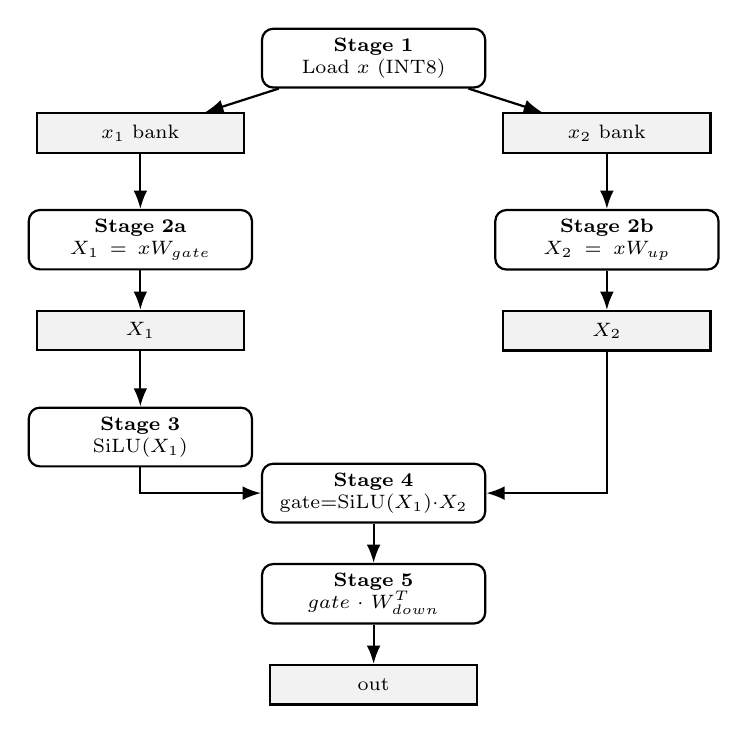
\begin{tikzpicture}[
    font=\scriptsize,
    >=Latex,
    node distance=5mm,
    block/.style={draw, rounded corners, thick, align=center, minimum height=6mm, text width=2.6cm},
    mem/.style={draw, thick, align=center, minimum height=5mm, text width=2.4cm, fill=gray!10},
    line/.style={-Latex, thick}
]

% Stage 1 (centered)
\node[block] (loadx) {\textbf{Stage 1}\\Load $x$ (INT8)};

% Split (tight + symmetric)
\node[mem, below left=3mm and 2mm of loadx] (x1buf) {$x_1$ bank};
\node[mem, below right=3mm and 2mm of loadx] (x2buf) {$x_2$ bank};

% Stage 2
\node[block, below=7mm of x1buf] (x1) {\textbf{Stage 2a}\\$X_1=xW_{gate}$};
\node[block, below=7mm of x2buf] (x2) {\textbf{Stage 2b}\\$X_2=xW_{up}$};

% Caches
\node[mem, below=of x1] (x1cache) {$X_1$};
\node[mem, below=of x2] (x2cache) {$X_2$};

% Stage 3 (left branch only)
\node[block, below=7mm of x1cache] (silu) {\textbf{Stage 3}\\SiLU($X_1$)};

% Stage 4 (CENTERED BETWEEN BRANCHES)
\node[block, below=10mm of $(silu)!0.5!(x2cache)$] (gate)
{\textbf{Stage 4}\\gate=SiLU($X_1$)$\cdot X_2$};

% Stage 5
\node[block, below=of gate] (down)
{\textbf{Stage 5}\\$gate \cdot W_{down}^{T}$};

% Output
\node[mem, below=of down] (out) {out};

% Connections
\draw[line] (loadx) -- (x1buf);
\draw[line] (loadx) -- (x2buf);

\draw[line] (x1buf) -- (x1);
\draw[line] (x2buf) -- (x2);

\draw[line] (x1) -- (x1cache);
\draw[line] (x2) -- (x2cache);

\draw[line] (x1cache) -- (silu);

% BOTH branches go DOWN into Stage 4
\draw[line] (silu.south) |- (gate.west);
\draw[line] (x2cache.south) |- (gate.east);

\draw[line] (gate) -- (down);
\draw[line] (down) -- (out);

\end{tikzpicture}
\caption{Compact dataflow of the SwiGLU accelerator.}
\label{fig:swiglu_compact}
\end{figure}



\section{Experiments} \label{sec:experiments}

\subsection{Experimental Setup}

\textbf{Hardware Platform.} Experiments were conducted on an embedded platform featuring a quad-core CPU running at 1.3\,GHz and an FPGA fabric operating at 250\,MHz. The system is equipped with 4\,GB of shared memory. Power measurements were obtained using onboard sensors sampling at runtime via the AMD \texttt{xmutil} toolchain.

\textbf{Software Stack.} The inference engine is based on a modified version of \texttt{llama.cpp}, extended to support hardware offloading of the SwiGLU block. Models are executed using Q4\_K quantization format. The FPGA accelerator was synthesized using Vitis high-level synthesis (HLS) toolchain.

\textbf{Workload.} The evaluation uses the LFM2.5-1.2B language backbone with input vectors of size 2048 and feed-forward dimension 8192. The accelerator processes one token per invocation, with multi-token prefill handled by sequential IP calls in the driver loop, issued by a modified \texttt{llama.cpp}. This reflects the single-token synthesis constraint imposed by on-chip memory limits. 

\subsection{Evaluation Metrics}

The evaluation considers the following metrics:

\begin{itemize}
    \item \textbf{Latency per token} ($\mu$s)
    \item \textbf{Throughput} (tokens/s)
    \item \textbf{Power consumption} (W)
    \item \textbf{Energy per token} (J/token)
    \item \textbf{Performance per watt} (tokens/s/W)
    \item \textbf{FPGA resource utilization} (LUT, FF, BRAM, URAM, DSP)
\end{itemize}

\subsection{Baseline Configuration}

The baseline corresponds to CPU Only execution of the same model using identical quantization settings and inference pipeline. In the accelerated configuration, only the SwiGLU block is offloaded to the FPGA, while all remaining operations are executed on the CPU.

\subsection{Results}

This section compares CPU Only and FPGA+CPU execution across thread counts (T1--T4) using throughput and performance-per-watt. Table~\ref{tab:results} reports the main quantitative results, while Fig.~\ref{fig:perf_w} and Fig.~\ref{fig:utilization} provide complementary views of efficiency trends and hardware resource usage.

\begin{table}[h]
\centering
\scriptsize
\caption{CPU Only vs FPGA+CPU results across thread counts (KV260).}
\label{tab:results}
\setlength{\tabcolsep}{3pt}
\begin{tabular}{c c c c c c}
\hline
Threads & Mode & Prefill (t/s) & Decode (t/s) & Prefill (t/s/W) & Decode (t/s/W) \\
\hline
T1 & CPU Only & 1.10 & 0.97 & 0.2300 & 0.2028 \\
T1 & FPGA+CPU & 1.83 & 1.53 & 0.3768 & 0.3150 \\
\hline
T2 & CPU Only & 2.19 & 1.07 & 0.4298 & 0.2100 \\
T2 & FPGA+CPU & 2.35 & 2.03 & 0.4683 & 0.4045 \\
\hline
T3 & CPU Only & 3.06 & 2.61 & 0.5102 & 0.4352 \\
T3 & FPGA+CPU & 2.55 & 2.22 & 0.4461 & 0.3883 \\
\hline
T4 & CPU Only & 3.27 & 2.51 & 0.6281 & 0.4821 \\
T4 & FPGA+CPU & 2.47 & 2.08 & 0.4885 & 0.4113 \\
\hline
\end{tabular}
\end{table}
\textbf{Key observations.} The FPGA+CPU path improves efficiency at lower thread counts, but not uniformly across all settings. At T1, performance-per-watt improves by +63.8\% (prefill) and +55.3\% (decode) versus CPU Only. At T2, gains are +9.0\% (prefill) and +92.6\% (decode). At higher thread counts, CPU Only remains superior in performance-per-watt: FPGA+CPU is lower by 12.6\%/10.8\% at T3 and 22.2\%/14.7\% at T4 (prefill/decode). Since board-level power remains close between modes, these trends indicate that end-to-end throughput is dominated by orchestration and memory movement effects rather than raw arithmetic scaling alone.

\begin{figure}[!ht]
  \centering
  
\includegraphics[width=\linewidth]{images/power_summary_T1_T4_perf_w.png}
  \caption{Obtained performance-per-watt in llama-bench for CPU Only execution at various thread counts, compared with FPGA+CPU.}
  \label{fig:perf_w}
\end{figure}

\begin{figure}[!ht]
  \centering
  \includegraphics[width=\linewidth]{images/utiliz.png}
  \caption{Utilization of the Kria KV260 on-board resources for the implementation of the feed-forward block accelerator.}
  \label{fig:utilization}
\end{figure}

\section{Discussion} \label{sec:discussion}
The experimental results show that offloading the SwiGLU feed-forward block to FPGA improves energy efficiency, even when absolute throughput does not consistently surpass the CPU Only baseline at higher thread counts. This is consistent with the design target: SwiGLU is a dominant kernel, and accelerating it reduces compute energy per token, especially in low-to-moderate CPU-thread regimes (e.g., T1/T2), where the FPGA+CPU configuration achieves better performance-per-watt. At higher thread counts (T3/T4), CPU Only execution remains faster, indicating that host-side overheads and memory-transfer costs still limit end-to-end speedup.

A key practical constraint is resource saturation in the programmable logic: most usable LUT/logic budget is already occupied, and additional parallelization attempts increase routing pressure and timing-closure difficulty rather than yielding proportional gains. The design is near the efficient frontier of this device for the current architecture. These findings reinforce that, for edge transformer inference, compute offload alone is not sufficient; optimizing weight movement, memory layout, and access/bandwidth orchestration is equally critical to convert kernel-level acceleration into full-system performance gains while preserving the observed energy-efficiency benefits.
\section{Conclusion} \label{sec:conclusion}
This work presented a selective FPGA offload strategy for LFM2.5-1.2B-Thinking, targeting the SwiGLU feed-forward block to enable conversational audio inference pipelines on resource-constrained edge platforms. The implementation integrates with the existing llama.cpp/ggml flow and demonstrates measurable energy-efficiency gains, especially at low and moderate thread counts, while preserving framework compatibility. Although the FPGA path does not consistently exceed CPU Only throughput at higher thread counts, the results clarify the limiting factors: practical on-device performance is jointly determined by compute parallelism, weight/data movement, and host-device orchestration. Importantly, the design already operates near the usable logic and routing budget of the target FPGA, so further gains are less likely to come from naive parallel replication and more likely from memory-path restructuring, overlap of transfers with compute, and tighter stage-level balancing (notably in stages 2 and 4). Overall, the study confirms that selective feed-forward acceleration is a viable and energy-effective step toward conversational-level edge inference, and provides a concrete roadmap for next optimizations in LFM2-Audio-1.5B deployment.
\bibliographystyle{IEEEtran}
\bibliography{bibliography.bib}

\end{document}
